% =====================================================================
%  Основное содержимое отчёта.
% =====================================================================

\labpart{Структура разработанной системы}

Система реализована как набор взаимодействующих по HTTP сервисов,
поднимаемых единой командой \texttt{docker compose up}. Внутри каждого
сервиса выдержано разделение на слои \texttt{domain} (чистая логика без
I/O), \texttt{application} (сценарии использования),
\texttt{infrastructure} (БД, HTTP-клиенты, обход веб-страниц) и
\texttt{interface} (маршруты FastAPI). Логика обработки естественного
языка (разбиение текста на слова, TF-IDF, косинусная мера, метрики)
вынесена в отдельную переиспользуемую библиотеку
\texttt{packages/nlp\_core}, не привязанную ни к одному сервису, а
\texttt{nlp-service} -- лишь тонкая HTTP-обёртка над ней; это и есть
углублённый элемент варианта -- модуль индексирования документов.
Дополнительно к обязательной для варианта векторной модели на TF-IDF в
этом же модуле реализована и вторая модель поиска -- на плотных
векторных представлениях документа и запроса, которые вычисляются
моделью Qwen3-Embedding-8B; она предназначена для сравнения качества
обоих подходов на одной и той же тестовой коллекции и представляет
собой дополнительное углубление этого элемента сверх минимальных
требований варианта.

Структура системы на уровне контейнеров (C4, уровень 2) показана на
рисунке~\ref{fig:architecture-c4}.
% Диаграмма общая для всех лабораторных работ курса: при переходе к
% ЛР2--4 в неё достаточно добавить новые Container(...)/Rel(...) в
% исходнике lab/diagrams/src/architecture-c4.puml, не перерисовывая всё
% заново.

\pumldiagram{architecture-c4}{Диаграмма контейнеров разработанной системы (нотация C4)}{architecture-c4}{0.85}

% Разбиение по зоне ответственности, а не по лабораторной работе,
% выбрано осознанно: последующие лабораторные работы курса (определение
% языка, реферирование, машинный перевод) подключаются к тем же
% таблицам documents/collections и к той же библиотеке nlp_core как
% новые сценарии использования, а не как копии инфраструктуры.

\labpartbreak{Структура базы данных}

Модель данных спроектирована как мультиколлекционная -- не «документы для
поиска», а «документы» вообще.
% Такое обобщение сделано, чтобы под ту же модель ложились и корпуса
% будущих лабораторных работ.
Схема ключевых таблиц и связей между ними показана на
рисунке~\ref{fig:database-erd} в нотации Crow's Foot.

\pumldiagram{database-erd}{ER-диаграмма базы данных (нотация Crow's Foot)}{database-erd}{1.0}

Пара \texttt{document\_terms.tf} + \texttt{term\_weights.weight} -- это
то, что в методических указаниях называется поисковым образом документа
(вектором документа); таблица \texttt{terms} с агрегатом
\texttt{COUNT(DISTINCT document\_id)} -- источник инверсной частоты
термина (формула 1.5). Таблицы \texttt{search\_models} и
\texttt{document\_chunk\_embeddings} хранят плотные векторные
представления для второй, эмбеддинговой модели поиска (Qwen3-Embedding-8B),
описанной выше; \texttt{crawl\_jobs}/\texttt{crawl\_urls} -- параметры и
живой прогресс выполнения задания на обход и очередь обхода (состояние
каждого URL: \texttt{queued}/\texttt{fetching}/\texttt{success}/
\texttt{failed}).

\labpart{Основные алгоритмы}

\textbf{Обход веб-страниц.} Обход выполняется по алгоритму поиска в
ширину (BFS) с ограничением по глубине и количеству документов.
Стартовые URL кладутся в \texttt{crawl\_urls} с \texttt{depth=0}; робот
извлекает из очереди URL с наименьшей глубиной, проверяет
\texttt{robots.txt} и ограничивает частоту запросов к одному домену,
скачивает и очищает текст, сохраняет документ и кладёт исходящие ссылки
в очередь с \texttt{depth+1}, если новая глубина не превышает
\texttt{max\_depth} и общий счётчик документов не превысил
\texttt{max\_documents}. Повторы исключаются по нормализованному URL в
рамках одного задания на обход.

\textbf{Предварительная обработка текста.} Текст документа проходит
очистку HTML, разбиение на предложения и слова, приведение к нижнему
регистру, удаление стоп-слов и лемматизацию (spaCy, модель
\texttt{en\_core\_web\_sm} для английского языка согласно варианту).

\textbf{Индексация.} Для каждого термина $i$ рассчитывается инверсная
частота
\begin{equation}
  B_i = \log\!\left(\frac{N}{P_i}\right),
\end{equation}
где $N$ -- число документов в коллекции, $P_i$ -- число документов,
содержащих термин $i$; вес термина в документе $j$ --
\begin{equation}
  A_i^{\,j} = Q_i^{\,j} \cdot B_i,
\end{equation}
где $Q_i^{\,j}$ -- частота термина $i$ в документе $j$ (TF). Итоговый
вектор документа $D$ -- вектор весов $A_i^{\,j}$, нормированный на
собственную евклидову норму; в обозначениях методических указаний (где
термин $k$, документ $d$, $N_{dk} \equiv Q_i^{\,j}$, $N_k \equiv P_i$)
это записывается как
\begin{equation}
  w_{dk} = \frac{N_{dk}\log(N / N_k)}{\sqrt{\sum_j \left(N_{dj}\log(N / N_j)\right)^2}},
\end{equation}
где сумма в знаменателе -- та же евклидова норма вектора весов документа
$d$, то есть числитель -- это $A_i^{\,j}$ из формулы (2), а всё выражение
-- нормированный $A_i^{\,j}$. Такая нормализация впоследствии позволяет
свести косинусную меру к скалярному произведению нормированных векторов.
Реализация этих формул -- чистые функции без побочных эффектов, покрытые
модульными тестами.

\textbf{Поиск.} Запросу пользователя ставится в соответствие бинарный
вектор $Q = \{w_{q1}, \dots, w_{qn}\}$, где $w_{qj} = 1$, если $j$-е
слово присутствует в запросе, и $w_{qj} = 0$ в противном случае -- то
есть вектор запроса не взвешивается по IDF, в отличие от вектора
документа. Мера схожести документа $D$ и запроса $Q$ вычисляется как
косинус угла между векторами:
\begin{equation}
  r(D,Q) = \frac{(D,Q)}{\lVert D \rVert \cdot \lVert Q \rVert},
\end{equation}
где $(D,Q)$ -- скалярное произведение векторов, $\lVert D \rVert$ и
$\lVert Q \rVert$ -- их евклидовы нормы. Документы сортируются по
убыванию $r(D,Q)$; в выдачу попадают топ-$K$ документов с фрагментом
текста (первые $\approx$300 символов), в котором подсвечены найденные
слова запроса.

\textbf{Оценка качества.} Метрики реализованы как чистые функции от
(ранжированный список, множество релевантных документов): Precision,
Recall, F1 на топ-$K$ (отдельно $K=5$ и $K=10$), Average Precision (AP),
R-Precision и 11-точечная интерполированная кривая Precision/Recall
(модуль \texttt{nlp\_core.metrics}), в соответствии с методикой ROMIP.

\labpart{Тестовая коллекция документов}

Для оценки качества собрана коллекция \texttt{GTA}: 1000 документов на
английском языке, 18\,071 уникальная лемма в словаре, средний объём
документа -- $\approx$11\,306 символов очищенного текста. Коллекция
наполнена двумя независимыми запусками обхода, каждый ограничен своим
доменом (\autoref{fig:collections}): с \texttt{grandtheftwiki.com}
(глубина 3, лимит 500 документов; получено 500 из 538 посещённых URL,
479 ошибок -- в основном служебные страницы редактирования и
обсуждения) и с \texttt{gta.wiki} (глубина 3, лимит 500 документов;
получено 500 из 539 посещённых URL, ошибок не было). Итоговая коллекция
и её документы также показаны на том же рисунке.

\begin{figure}[H]
  \centering
  \begin{subfigure}{0.48\textwidth}
    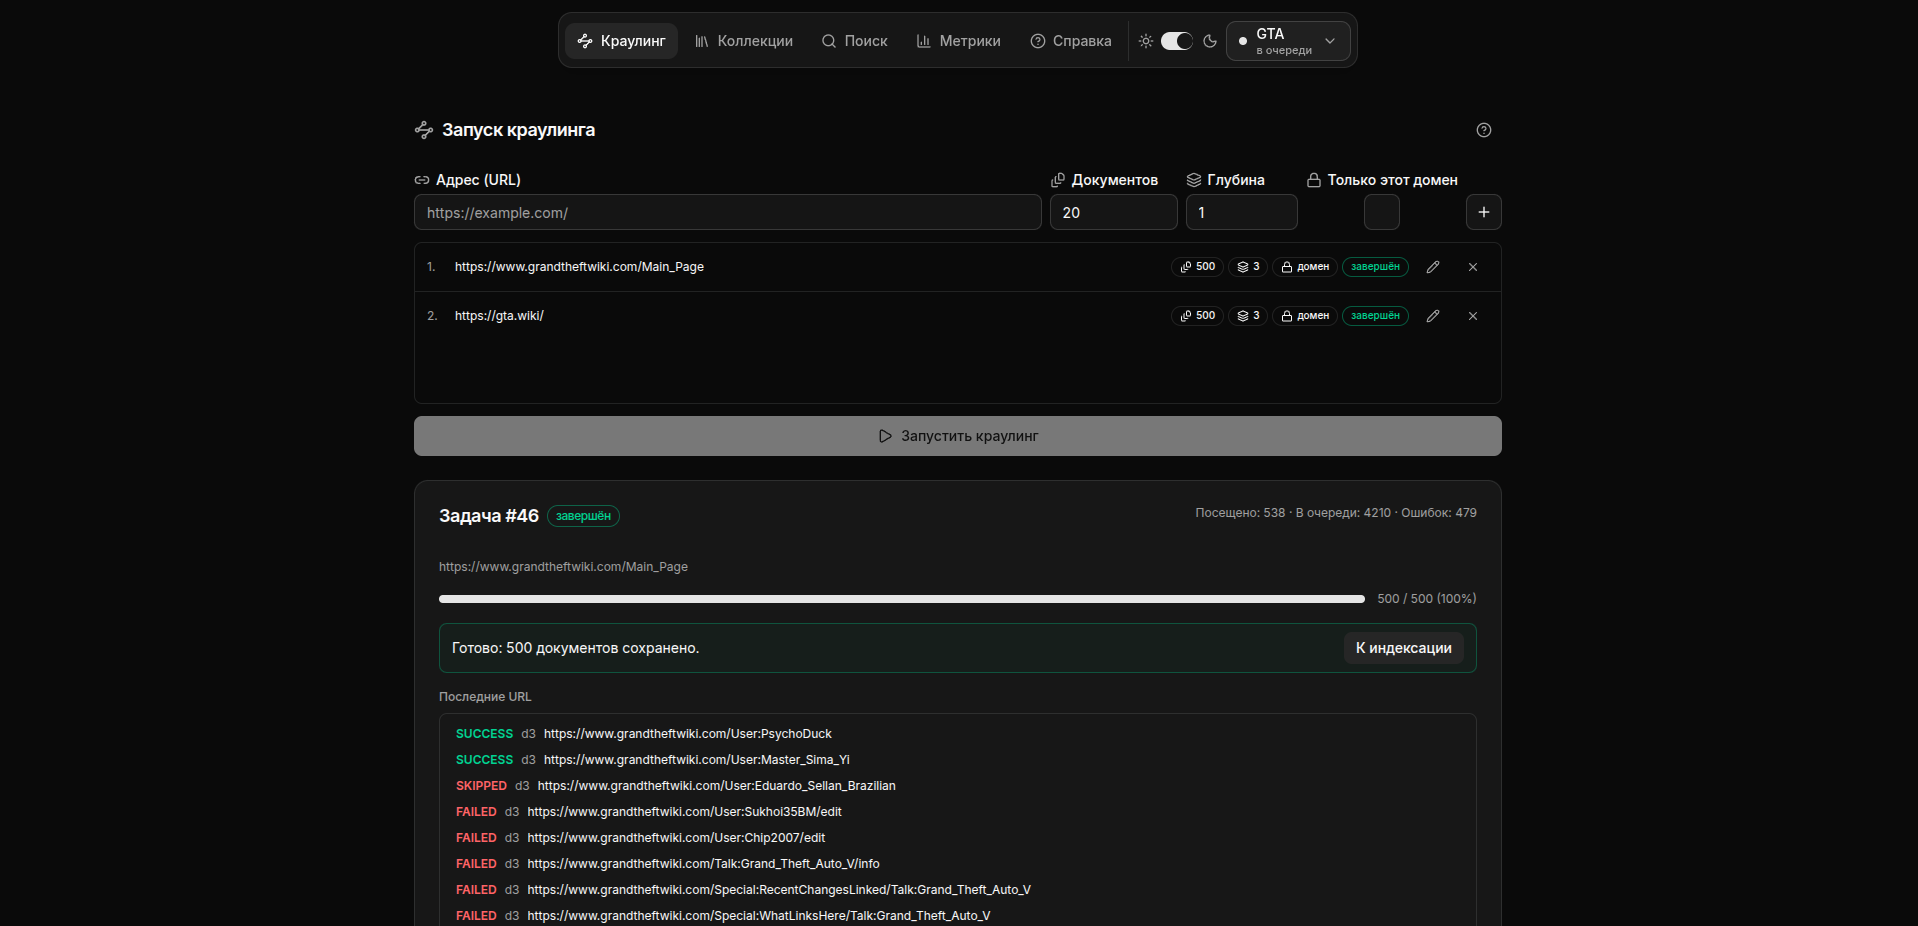
\includegraphics[width=\linewidth]{lab/pictures/crawling.png}
    \caption{Запуск обхода}
  \end{subfigure}
  \hfill
  \begin{subfigure}{0.48\textwidth}
    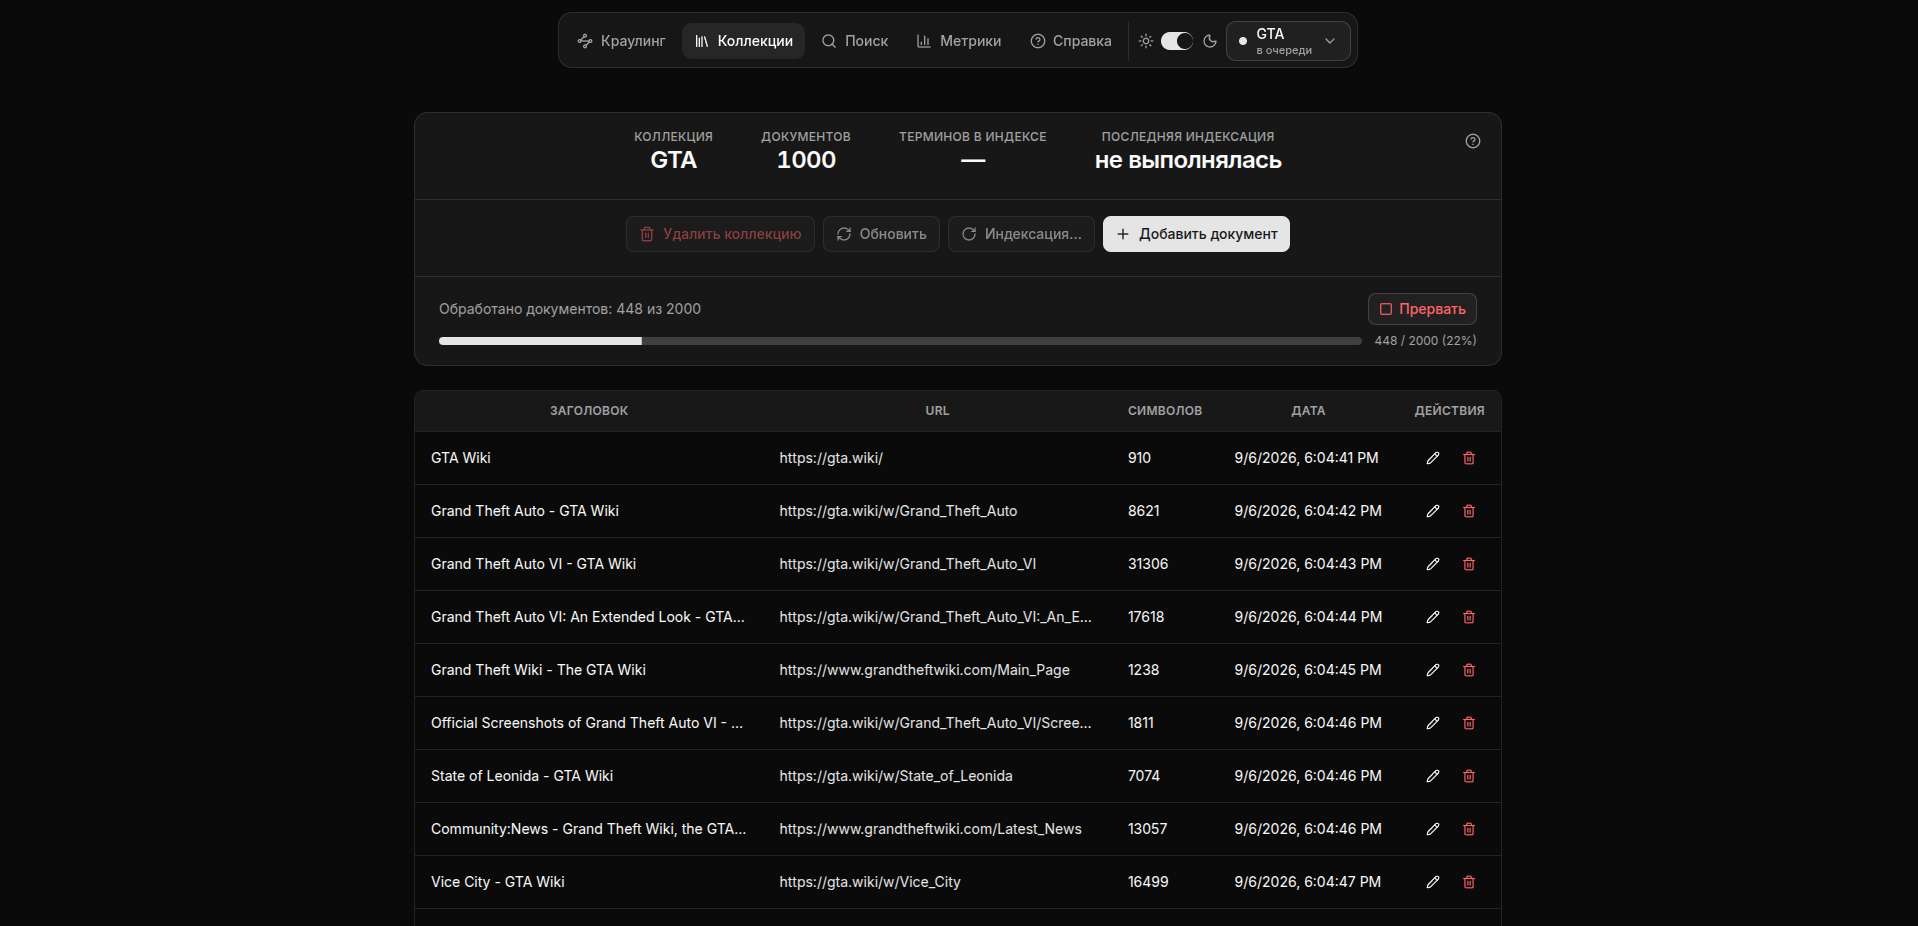
\includegraphics[width=\linewidth]{lab/pictures/collections.png}
    \caption{Наполненная коллекция}
  \end{subfigure}
  \caption{Сбор тестовой коллекции \texttt{GTA} в интерфейсе системы}
  \label{fig:collections}
\end{figure}

Для коллекции сформулировано 5 тестовых запросов на английском языке:
\textit{GTA series publisher}, \textit{GTA 5 first day sales volume},
\textit{GTA VI release date}, \textit{Vice City highway system},
\textit{Megamundo building}. Для каждого запроса выполнен поиск обеими
реализованными моделями (TF-IDF и Qwen3-Embedding-8B), и в режиме
разметки на странице «Поиск» отмечены документы, признанные
релевантными (\autoref{fig:search}) -- итого 32 отметки (12, 3, 8, 4 и 5
документов по перечисленным запросам соответственно), хранящиеся в
таблице \texttt{relevance\_judgments}. Интерфейс поддерживает только
положительную отметку «релевантно»; все остальные документы из выдачи,
не отмеченные пользователем, считаются нерелевантными при расчёте
метрик.

\begin{figure}[H]
  \centering
  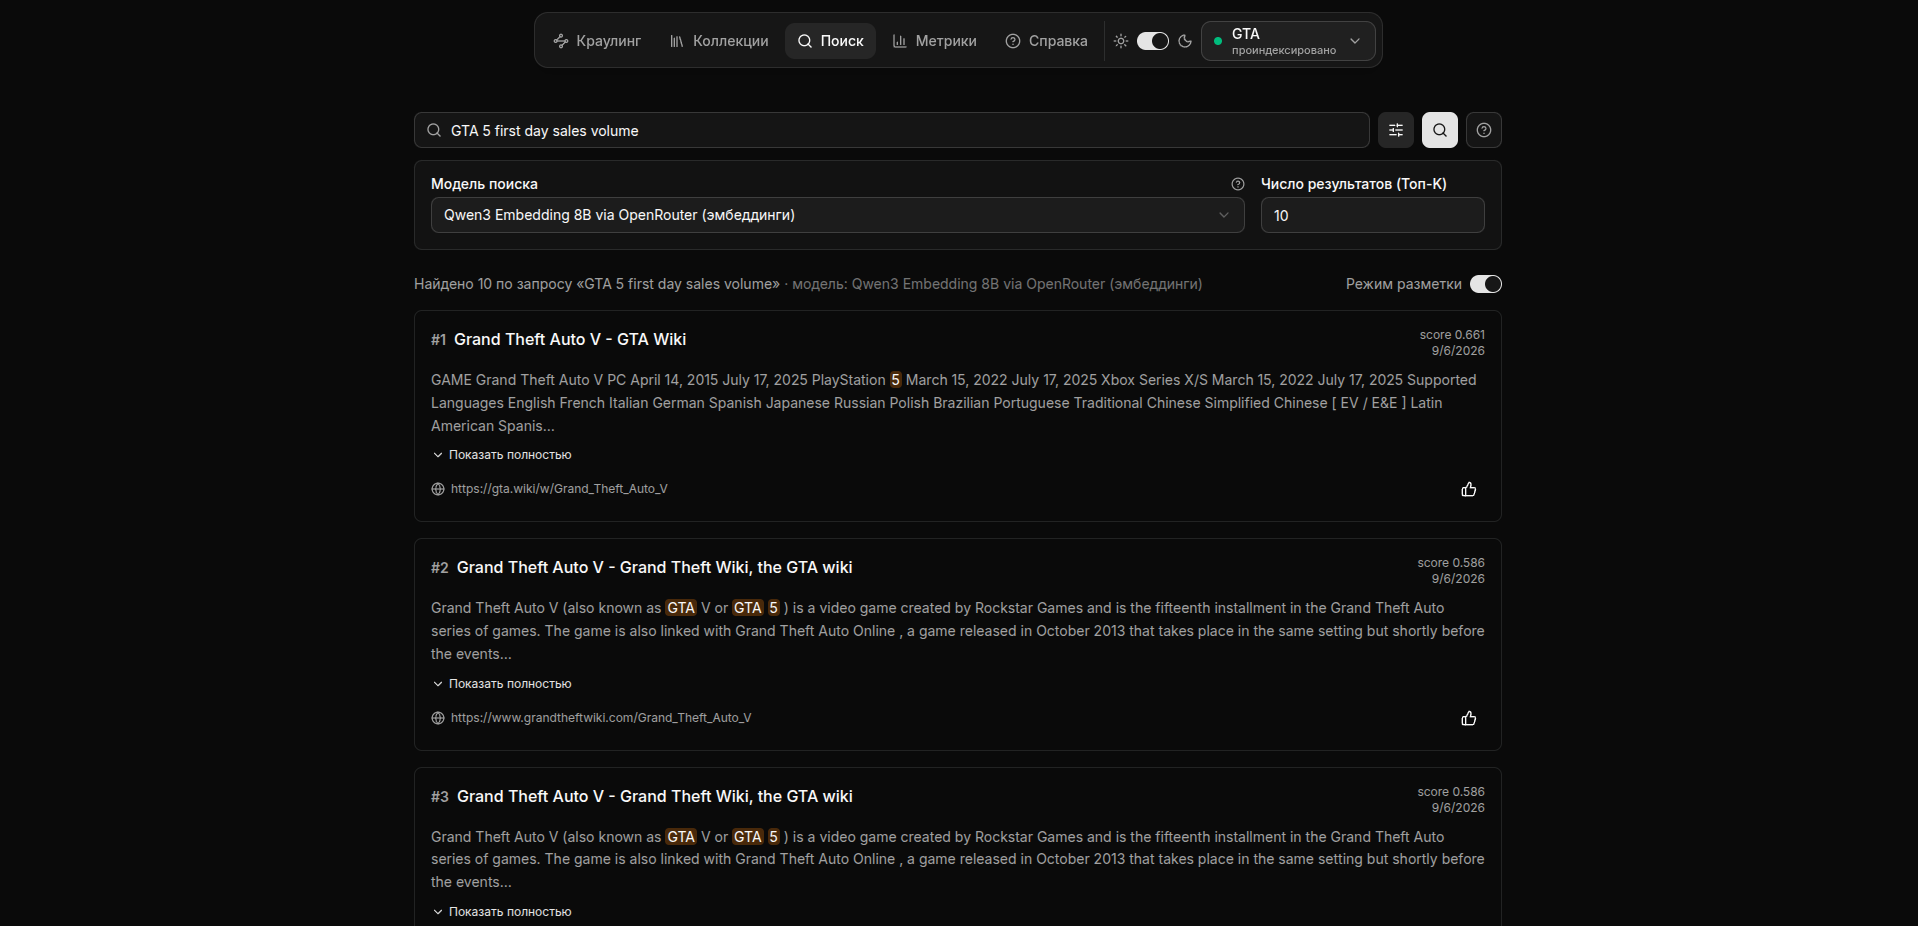
\includegraphics[width=0.8\textwidth]{lab/pictures/search.png}
  \caption{Поиск по коллекции с выбором модели и разметкой релевантности}
  \label{fig:search}
\end{figure}

\labpart{Результаты оценки по метрикам}

Метрики посчитаны для обеих реализованных моделей поиска -- обязательной
(TF-IDF + косинусная мера) и дополнительной (Qwen3-Embedding-8B через
OpenRouter) -- на одной и той же тестовой коллекции \texttt{GTA} и одном
и том же наборе из 5 размеченных запросов; ни один запрос не пришлось
исключать из агрегатов -- у каждого нашёлся хотя бы один документ,
отмеченный релевантным. Средние по запросам значения приведены в
таблице~\ref{tab:metrics-gta}; тот же расчёт в интерфейсе системы -- на
рисунке~\ref{fig:metrics-ui}.

\begin{table}[H]
  \centering
  \caption{Средние метрики качества по 5 тестовым запросам коллекции \texttt{GTA}}
  \label{tab:metrics-gta}
  \begin{tabularx}{\textwidth}{|X|r|r|}
    \hline
    Метрика & TF-IDF + косинусная мера & Qwen3-Embedding-8B \\
    \hline
    MAP & 0{,}442 & 0{,}842 \\
    \hline
    R-Precision & 0{,}475 & 0{,}775 \\
    \hline
    P@5 & 0{,}520 & 0{,}760 \\
    \hline
    P@10 & 0{,}300 & 0{,}580 \\
    \hline
    R@5 & 0{,}450 & 0{,}658 \\
    \hline
    R@10 & 0{,}492 & 0{,}950 \\
    \hline
    F1@5 & 0{,}465 & 0{,}666 \\
    \hline
    F1@10 & 0{,}358 & 0{,}681 \\
    \hline
  \end{tabularx}
\end{table}

\begin{figure}[H]
  \centering
  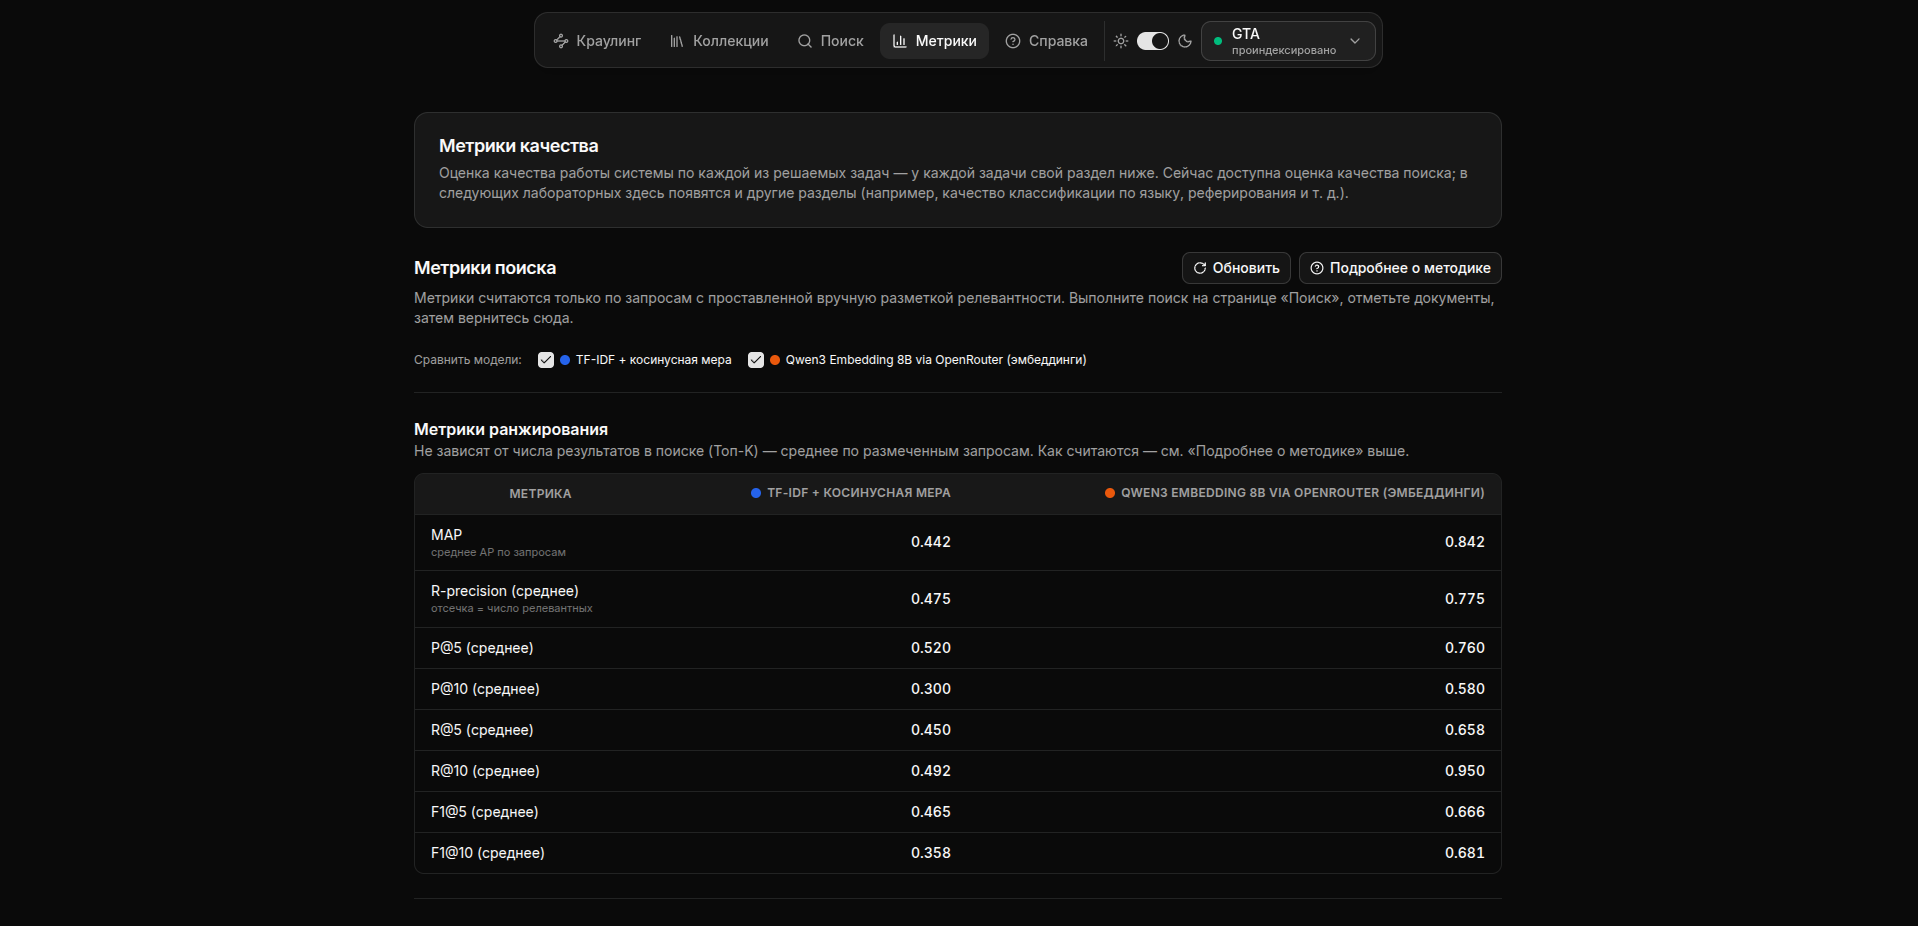
\includegraphics[width=0.8\textwidth]{lab/pictures/metrics.png}
  \caption{Таблица метрик качества поиска в интерфейсе системы}
  \label{fig:metrics-ui}
\end{figure}

Графическое представление метрик по каждому из 5 запросов -- на
рисунках~\ref{fig:bars-1} и~\ref{fig:bars-2} (синий -- TF-IDF, оранжевый
-- Qwen3-Embedding-8B).

\begin{figure}[H]
  \centering
  \begin{subfigure}{0.48\textwidth}
    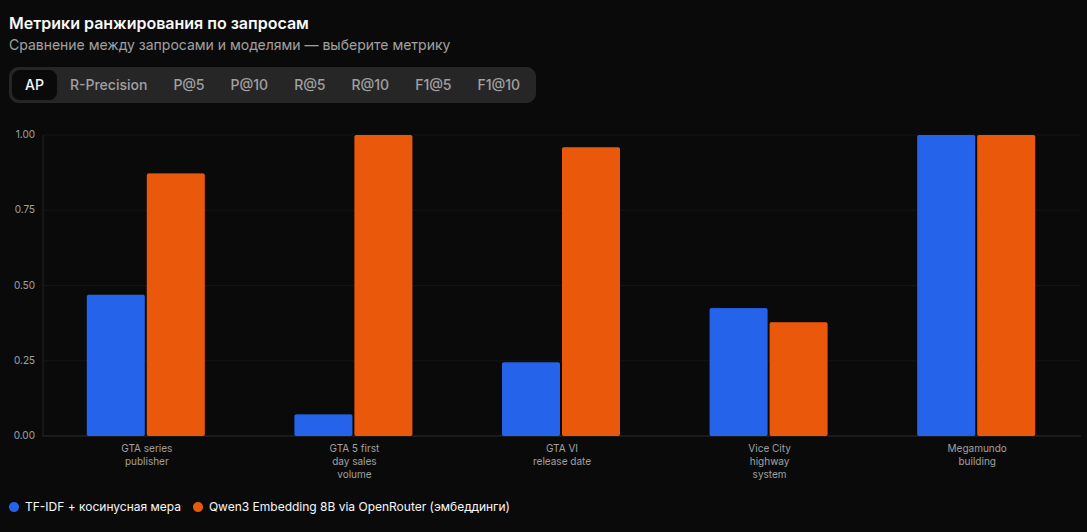
\includegraphics[width=\linewidth]{lab/pictures/ap_bar_chart.png}
    \caption{AP}
  \end{subfigure}
  \hfill
  \begin{subfigure}{0.48\textwidth}
    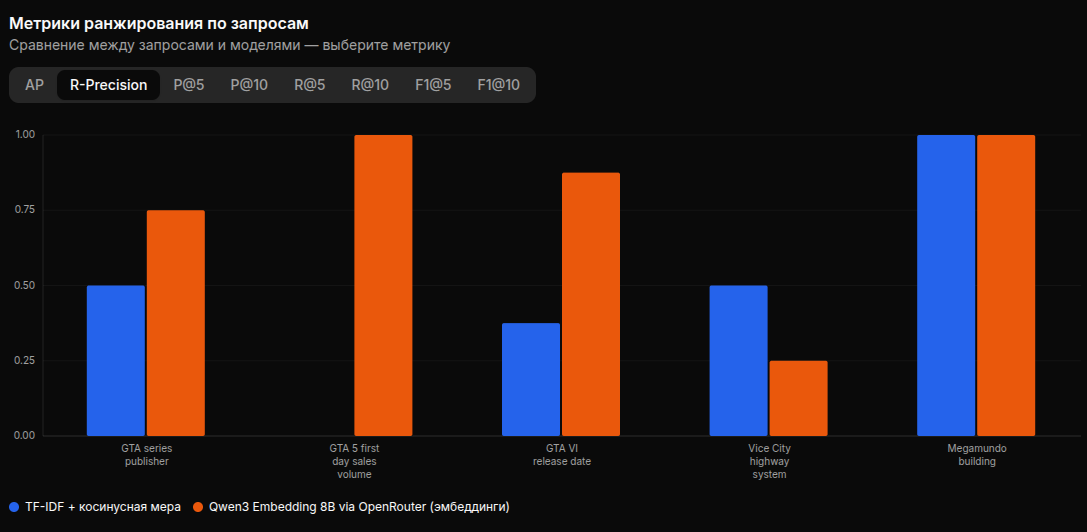
\includegraphics[width=\linewidth]{lab/pictures/r_precision_bar_chart.png}
    \caption{R-Precision}
  \end{subfigure}

  \vspace{0.5em}
  \begin{subfigure}{0.48\textwidth}
    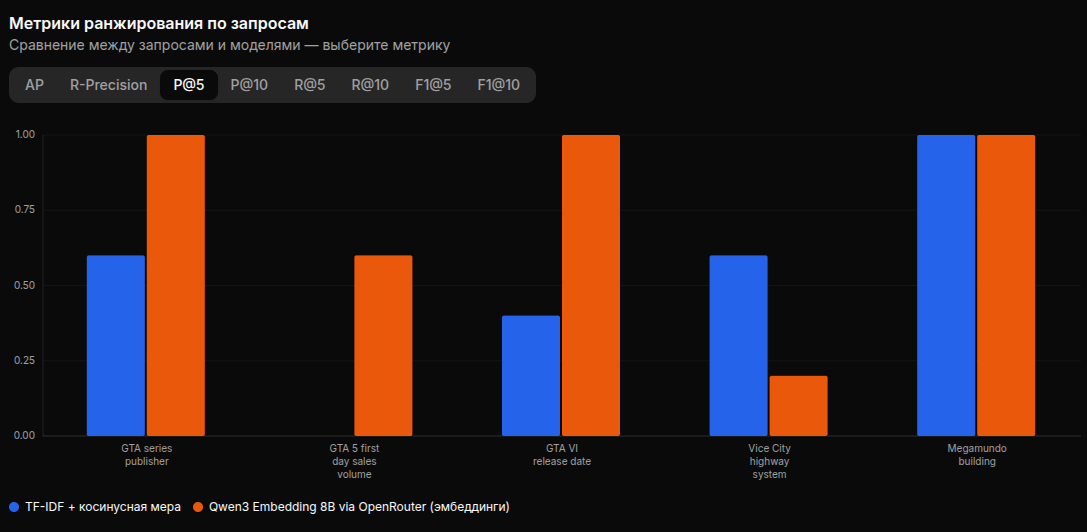
\includegraphics[width=\linewidth]{lab/pictures/p5_bar_chart.png}
    \caption{P@5}
  \end{subfigure}
  \hfill
  \begin{subfigure}{0.48\textwidth}
    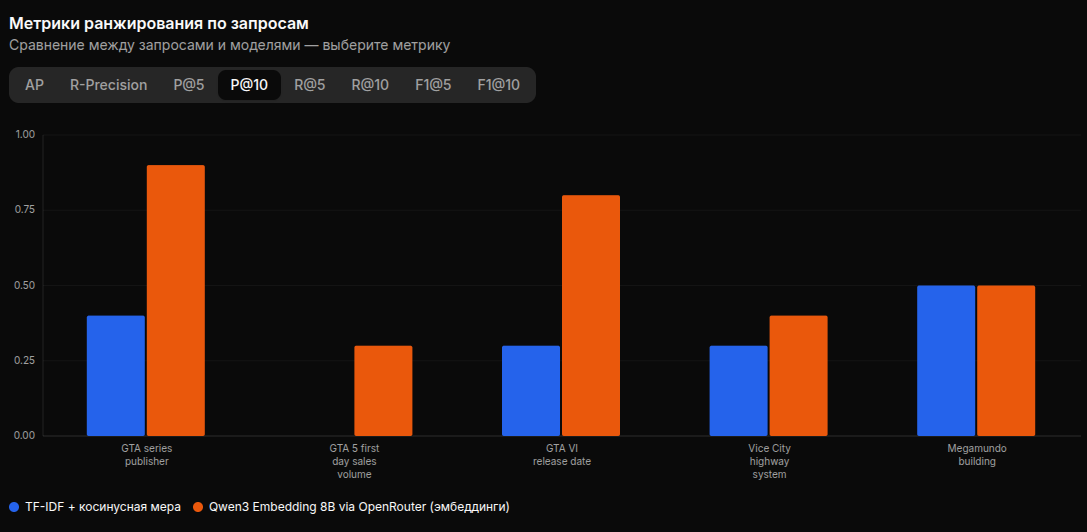
\includegraphics[width=\linewidth]{lab/pictures/p10_bar_chart.png}
    \caption{P@10}
  \end{subfigure}
  \caption{Метрики ранжирования по запросам: AP, R-Precision, P@5, P@10}
  \label{fig:bars-1}
\end{figure}

\begin{figure}[H]
  \centering
  \begin{subfigure}{0.48\textwidth}
    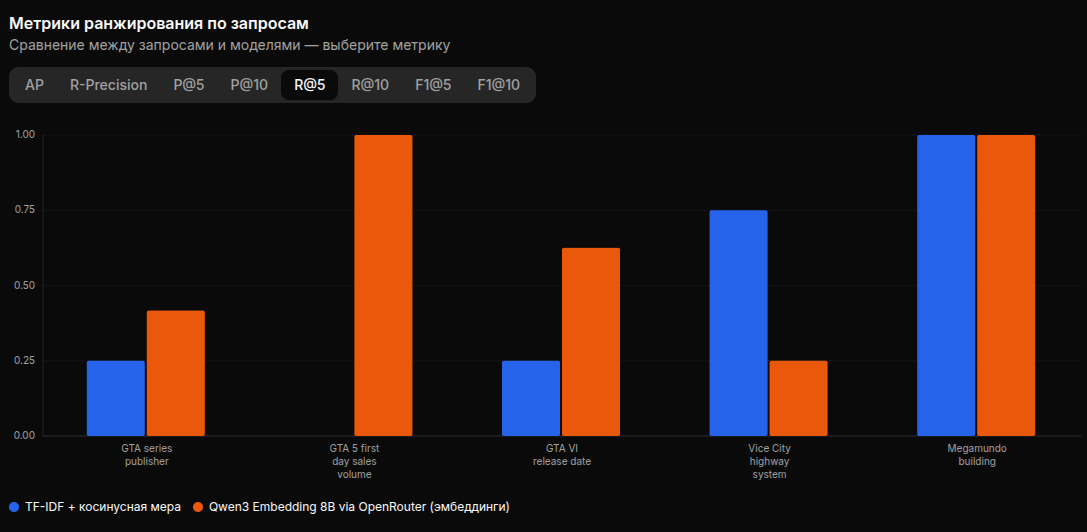
\includegraphics[width=\linewidth]{lab/pictures/r5_bar_chart.png}
    \caption{R@5}
  \end{subfigure}
  \hfill
  \begin{subfigure}{0.48\textwidth}
    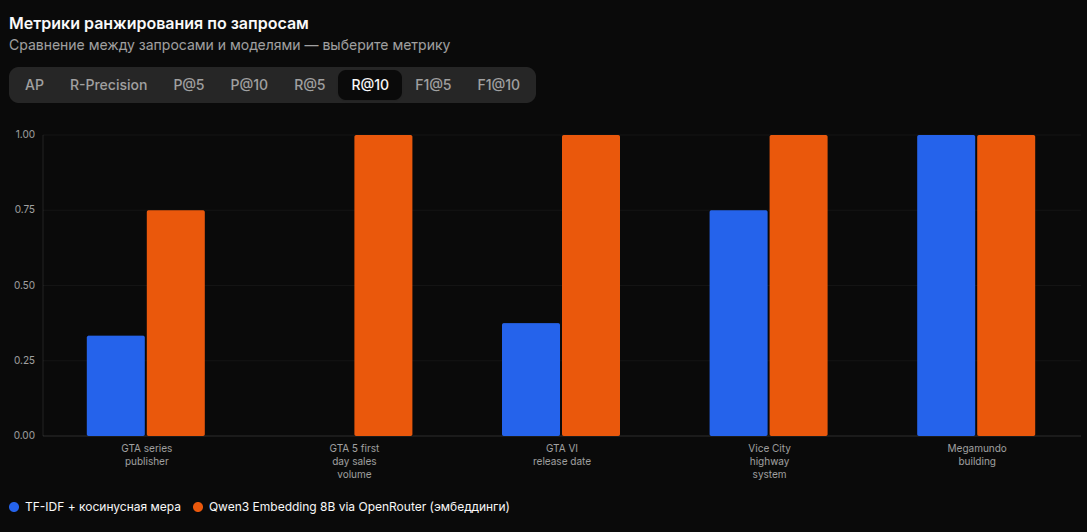
\includegraphics[width=\linewidth]{lab/pictures/r10_bar_chart.png}
    \caption{R@10}
  \end{subfigure}

  \vspace{0.5em}
  \begin{subfigure}{0.48\textwidth}
    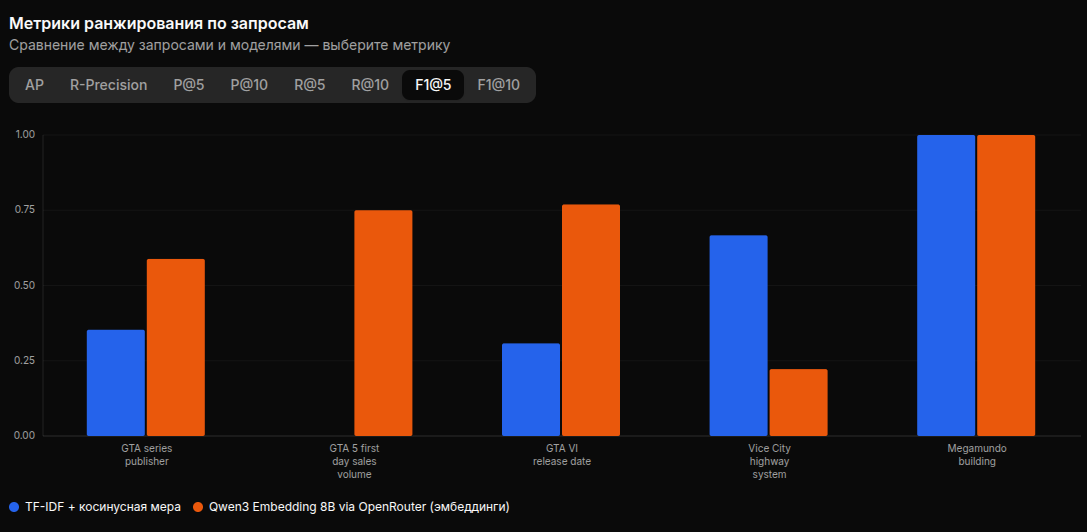
\includegraphics[width=\linewidth]{lab/pictures/f15_bar_chart.png}
    \caption{F1@5}
  \end{subfigure}
  \hfill
  \begin{subfigure}{0.48\textwidth}
    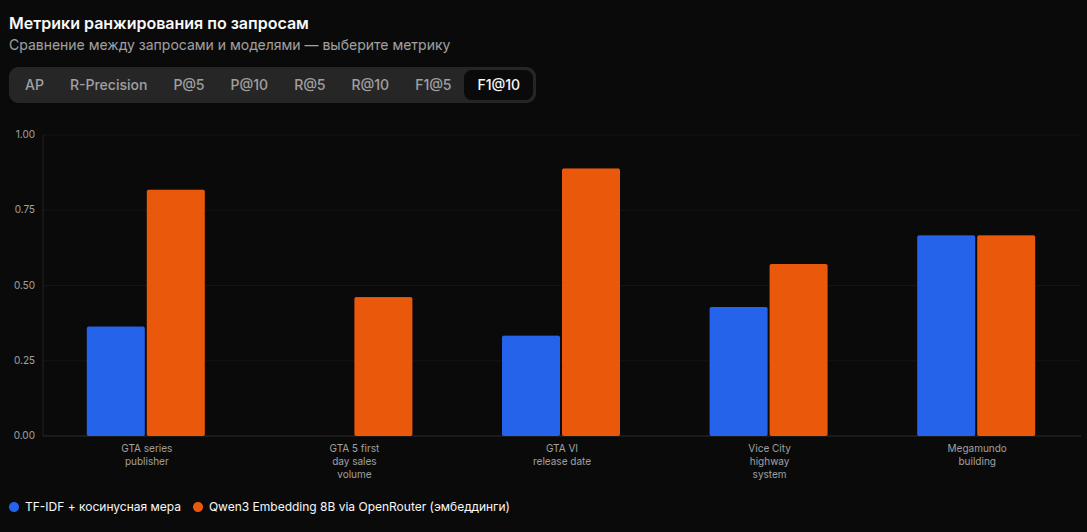
\includegraphics[width=\linewidth]{lab/pictures/f110_bar_chart.png}
    \caption{F1@10}
  \end{subfigure}
  \caption{Метрики ранжирования по запросам: R@5, R@10, F1@5, F1@10}
  \label{fig:bars-2}
\end{figure}

11-точечная интерполированная кривая Precision/Recall, усреднённая по
размеченным запросам, показана на рисунке~\ref{fig:trec-curve}: кривая
Qwen3-Embedding-8B лежит выше кривой TF-IDF практически на всём
диапазоне полноты, кроме самого высокого уровня, где обе модели
сближаются.

\begin{figure}[H]
  \centering
  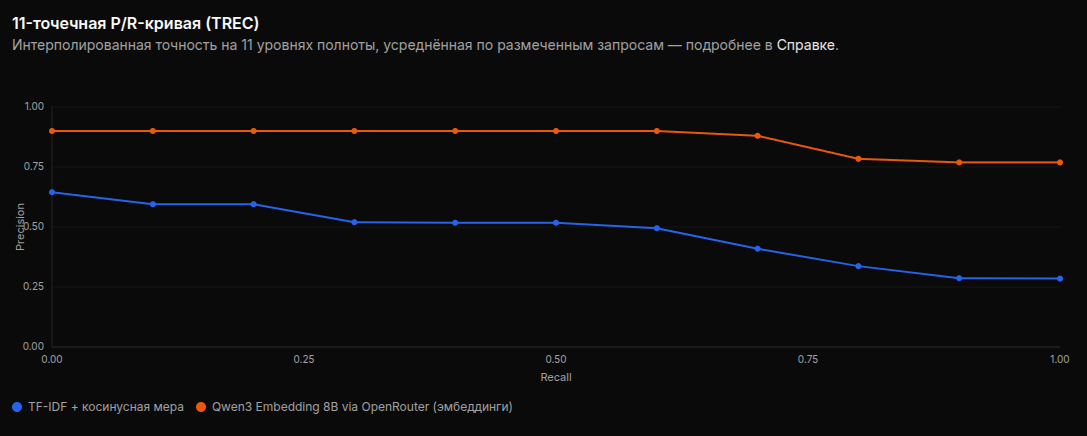
\includegraphics[width=0.8\textwidth]{lab/pictures/trec_curve.png}
  \caption{11-точечная интерполированная кривая Precision/Recall}
  \label{fig:trec-curve}
\end{figure}

\labpart{Анализ результатов и предложения по улучшению}

\begin{enumerate}
  \item \textbf{Эмбеддинговая модель в среднем точнее обязательной.}
  Qwen3-Embedding-8B превосходит TF-IDF по всем восьми агрегированным
  метрикам (\autoref{tab:metrics-gta}): MAP 0{,}842 против 0{,}442,
  R-Precision 0{,}775 против 0{,}475 и так далее. Ожидаемый результат:
  векторные представления учитывают смысл запроса, а не только
  буквальное совпадение слов с текстом документа.
  \item \textbf{Главный источник разрыва -- рассинхрон словаря
  (vocabulary mismatch).} На запросе \textit{"GTA 5 first day sales
  volume"} TF-IDF находит единственный релевантный документ только на
  дальних позициях выдачи (P@5 = P@10 = 0, AP = 0{,}07), тогда как
  Qwen -- уже в топ-5 (AP = 1{,}00, \autoref{fig:bars-1}). Страница,
  видимо, описывает продажи другими словами (например, суммой выручки
  вместо "sales volume"), не пересекающимися буквально с текстом
  запроса, -- TF-IDF в принципе не может найти документ без общих
  термов, а эмбеддинги устойчивы к такой перефразировке.
  \item \textbf{Но не всегда эмбеддинги выигрывают.} На запросе
  \textit{"Vice City highway system"} TF-IDF обходит Qwen по всем
  метрикам (P@5 0{,}60 против 0{,}20, AP 0{,}42 против 0{,}38,
  R-Precision 0{,}50 против 0{,}25) -- для узких формулировок,
  дословно совпадающих с текстом страницы, точное совпадение термов
  оказывается надёжнее семантического сходства. Предложение:
  реализовать гибридное ранжирование (например, взвешенную сумму или
  reciprocal rank fusion косинусных оценок обеих моделей), чтобы не
  терять точность на подобных запросах.
  \item \textbf{Что можно добавить в систему для её улучшения.}
  \begin{itemize}
    \item расширение запроса синонимами и близкими по смыслу словами
    (например, через векторы слов spaCy или WordNet) -- частично закрыло
    бы разрыв словаря из п.~б без отказа от быстрой и прозрачной модели
    на TF-IDF;
    \item переход от бинарной релевантности к градуированной шкале и
    метрике nDCG, чтобы различать «точное совпадение» и «частично по
    теме», а не только «релевантно / нерелевантно»;
    \item приближённый индекс поиска по векторным представлениям
    (\texttt{ivfflat}/\texttt{hnsw} в pgvector) -- сейчас поиск по
    эмбеддингам выполняется полным перебором, что приемлемо только для
    учебного масштаба коллекции;
    \item полуавтоматическое пополнение эталонной разметки -- объединение
    (pooling) топ-$K$ выдачи обеих моделей в единый список кандидатов на
    разметку, чтобы быстрее набрать рекомендованные методикой 15--20
    тестовых запросов, не размечая вручную каждый документ с нуля;
    \item многопользовательский режим с сохранением истории запросов и
    персональной разметкой, если систему развивать за пределы учебного
    проекта.
  \end{itemize}
  \item \textbf{Где систему можно применить.}
  \begin{itemize}
    \item внутрикорпоративный поиск по базе знаний или документации --
    коллекция и краулинг уже спроектированы так, чтобы наполняться из
    произвольного набора стартовых страниц одного источника (как
    коллекция \texttt{GTA} наполнена с \texttt{gta.wiki} и
    \texttt{grandtheftwiki.com});
    \item поиск по тематическим wiki-сайтам и базам знаний, где важна
    устойчивость к перефразировкам запроса пользователя -- здесь
    особенно уместна эмбеддинговая модель (п.~а);
    \item управляемый сбор и полнотекстовый поиск по узкой предметной
    области сети Интернет (мониторинг новостей по теме, дайджесты) --
    за счёт ограничения краулинга по домену и глубине обхода;
    \item учебный полигон для последующих лабораторных работ курса
    (определение языка, реферирование, машинный перевод, синтез и
    распознавание речи) -- архитектура и модель данных уже
    мультиколлекционные и переиспользуемые, без необходимости
    поднимать отдельную инфраструктуру под каждую лабораторную.
  \end{itemize}
\end{enumerate}

\labpart{Использованные готовые компоненты}

\begin{table}[H]
  \centering
  \caption{Библиотеки и программные средства, использованные при реализации}
  \label{tab:stack}
  \small
  \begin{tabularx}{\textwidth}{|l|X|}
    \hline
    Компонент & Назначение \\
    \hline
    FastAPI & Асинхронная библиотека для построения API, автоматическая
      генерация OpenAPI-схемы для клиентского приложения. \\
    \hline
    spaCy (\texttt{en\_core\_web\_sm}) & Разбиение текста на слова,
      лемматизация, удаление стоп-слов, определение частей речи для
      английского языка. \\
    \hline
    PostgreSQL + pgvector & Реляционное хранилище термов, весов и
      документов; расширение \texttt{pgvector} хранит плотные
      векторные представления документов и запросов для второй модели
      поиска (Qwen3-Embedding-8B), реализованной для сравнения с
      обязательной моделью на TF-IDF. \\
    \hline
    Alembic & Версионирование схемы базы данных. \\
    \hline
    httpx + BeautifulSoup & HTTP-клиент и разбор HTML для поискового
      робота. \\
    \hline
    React + Vite + TypeScript & Клиентское веб-приложение. \\
    \hline
    pytest & Модульное тестирование доменного слоя (\texttt{nlp\_core})
      без поднятия инфраструктуры. \\
    \hline
    Docker Compose & Единая среда запуска всех сервисов и базы данных. \\
    \hline
  \end{tabularx}
\end{table}

Требование методических указаний о доступном интерфейсе со
справочными подсказками реализовано отдельной страницей «Справка»
(\autoref{fig:help}): она описывает типичный порядок действий и
назначение каждой страницы приложения.

\begin{figure}[H]
  \centering
  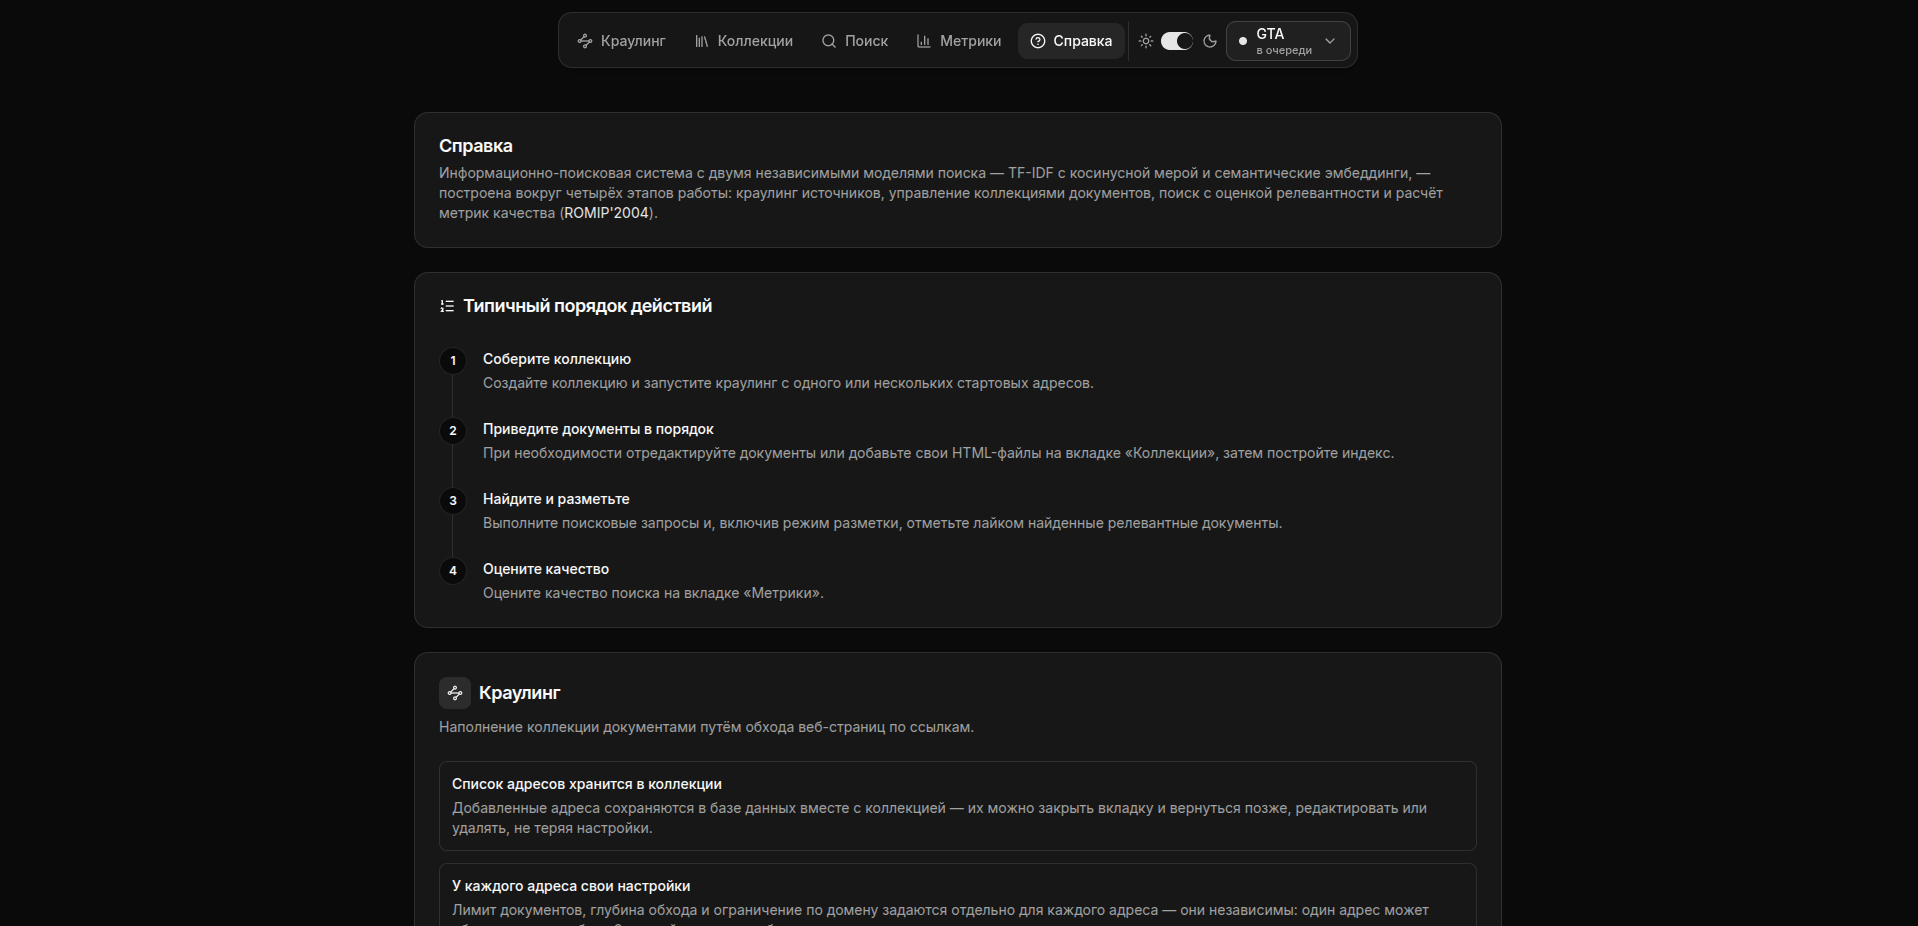
\includegraphics[width=0.8\textwidth]{lab/pictures/help.png}
  \caption{Страница «Справка» интерфейса системы}
  \label{fig:help}
\end{figure}
